\documentclass[12pt,letterpaper]{article}

% Layout exigido pela Behavior Research Methods (APA 7th ed.)
\usepackage[margin=1in]{geometry}
\usepackage{setspace}
\doublespacing
\usepackage{times}
\usepackage{microtype}
\usepackage{fancyhdr}
\setlength{\headheight}{15pt}
\pagestyle{fancy}
\fancyhf{}
\renewcommand{\headrulewidth}{0pt}
\rhead{\thepage}

% Matemática, tabelas e código
\usepackage[utf8]{inputenc}
\usepackage[T1]{fontenc}
\usepackage{amsmath,amssymb,bm}
\usepackage{booktabs}
\usepackage{array}
\usepackage{graphicx}
\usepackage{tikz} 
\usetikzlibrary{arrows.meta, positioning, fit, backgrounds}
\usepackage{xcolor}
\usepackage{listings}
\lstset{
  language=Python,
  basicstyle=\ttfamily\small\singlespacing,
  keywordstyle=\color{blue!70!black}\bfseries,
  stringstyle=\color{teal!70!black},
  commentstyle=\color{gray}\itshape,
  frame=tb,
  breaklines=true,
  columns=fullflexible,
  showstringspaces=false
}
\usepackage[colorlinks=true, allcolors=blue]{hyperref}

% Citações e referências em APA 7ª edição
\usepackage[style=apa, backend=biber]{biblatex}
\addbibresource{references.bib}

\begin{document}

% ==================== TITLE PAGE ====================
\begin{titlepage}
\centering
\vspace*{1.5cm}

{\Large \textbf{anvala: Numerical Parity with R and GPU-Accelerated Resampling for Latent Variable and Network Psychometrics in Python}\par}

\vspace{1.2cm}

{\large Frederico Gonçalves Pedrosa\textsuperscript{1}\par}

\vspace{0.6cm}

{\normalsize
\textsuperscript{1}Escola de Música, Universidade Federal de Minas Gerais (UFMG), Belo Horizonte, MG, Brazil\par
}

\vspace{1.5cm}

\begin{flushleft}
\textbf{Author Note}\\[4pt]
Frederico Gonçalves Pedrosa \url{https://orcid.org/0000-0002-0682-0734}\\
This work was supported by the Conselho Nacional de Desenvolvimento Científico e Tecnológico (CNPq, Brazil). The author declares no conflicts of interest.\\[8pt]
Correspondence concerning this article should be addressed to Frederico Gonçalves Pedrosa, Escola de Música, Universidade Federal de Minas Gerais (UFMG), Av. Pres. Antônio Carlos, 6627, Pampulha, Belo Horizonte, MG, 31270-901, Brazil. Phone: +55 (31) 3409-4700. E-mail: frederico.musicoterapia@gmail.com
\end{flushleft}
\end{titlepage}

% ==================== ABSTRACT ====================
\section*{Abstract}
\noindent Psychometric modeling has traditionally relied on R packages such as \texttt{lavaan}, \texttt{semTools}, and \texttt{EGAnet}, whereas modern computational and generative psychometrics---leveraging large language models, dense text embeddings, and tensor operations---operates primarily in Python. Moving data and models across both environments introduces workflow friction, serialization overhead, and reproducibility risks, while resampling-intensive procedures such as bias-corrected and accelerated (\texttt{BCa}) bootstrapping and bootstrap Exploratory Graph Analysis (\texttt{boot\_ega}) remain computationally expensive on sequential processors. We introduce \texttt{anvala} (v0.1.0), an open-source Python library built on PyTorch that delivers numerical parity with established R psychometric packages alongside graphics processing unit (GPU) tensor parallelization for resampling workflows. Using double-precision (\texttt{float64}) automatic differentiation and \texttt{lavaan}-compatible syntax, \texttt{anvala} implements continuous (\texttt{ML}, \texttt{MLR}) and ordinal (\texttt{WLSMV}) structural equation modeling, multi-group measurement invariance with partial invariance and Lagrange multiplier score tests, bifactor indices, and network psychometrics (\texttt{EGA}, Unique Variable Analysis, and entropy fit indices). Across canonical datasets, \texttt{anvala} reproduces R reference parameters, robust standard errors, scaled fit indices, and network structures within $10^{-16}$ to $10^{-5}$ across factor, ordinal, multi-group, bifactor, and network models (and within $1.10 \times 10^{-4}$ on the small-sample full SEM). Three simulation studies map the architectural crossover between CPU and GPU execution across model dimensionality ($p \in [3, 60]$) and verify $100\%$ convergence, low parameter bias ($< 5\%$), well-calibrated interval coverage, and unbiased latent mean recovery under partial invariance.

\vspace{0.5cm}
\noindent \textit{Keywords:} psychometrics, structural equation modeling, exploratory graph analysis, automatic differentiation, GPU acceleration, Python
\newpage

% ==================== INTRODUCTION ====================
\section{Introduction}

Latent variable models and network psychometrics are foundational analytical tools in psychological, educational, and clinical measurement. Confirmatory factor analysis (CFA), structural equation modeling (SEM), and multi-group invariance testing allow researchers to evaluate latent construct structures, compare groups, and estimate indirect effects while accounting for measurement error \parencite{bollen1989, byrne1989, muthen1984}. Alongside these latent variable frameworks, Exploratory Graph Analysis (EGA) represents psychological constructs as regularized partial correlation networks to estimate dimensionality and item stability without imposing a priori simple-structure constraints \parencite{christensen2021, epskamp2018, golino2017}. In applied research, these procedures are predominantly executed in R using mature, rigorously validated packages such as \texttt{lavaan} \parencite{rosseel2012}, \texttt{semTools} \parencite{jorgensen2026}, \texttt{EGAnet} \parencite{golino2017}, and \texttt{BifactorIndicesCalculator} \parencite{dueber2021}.

In recent years, however, psychometric methodology has increasingly integrated machine learning, dense semantic embeddings, and large language models (LLMs) into instrument development and structural validation \parencite{vondavier2021}. Within this rapidly growing line of computational and generative psychometrics, researchers leverage transformer architectures and embedding spaces to generate candidate items, screen semantic redundancy, simulate factor structures, and evaluate construct dimensionality prior to empirical data collection \parencite{hommel2022, kjell2019, russelllasalandra2026, urban2021, wulff2025}.

Because the core infrastructure for language modeling, embedding extraction, and tensor computation---such as PyTorch \parencite{paszke2019}---is developed natively in Python, which has also become a primary programming language in behavioral science \parencite{peirce2019}, researchers combining computational pipelines with classical psychometrics face an awkward cross-language split. Typical workflows require generating items or extracting embeddings in Python, serializing intermediate tables or invoking foreign-function bridges (e.g., \texttt{rpy2}) to estimate CFA, invariance, or EGA models in R, and re-importing outputs back into Python. Switching runtimes adds dependency fragility, complicates version control, and impedes iterative modeling.

Existing native Python packages do not yet provide the breadth or numerical fidelity needed to eliminate this cross-language dependency. General-purpose statistical libraries lack latent variable estimation altogether. Specialized packages such as \texttt{semopy} \parencite{igolkina2020} support continuous SEM estimation in Python, but do not implement ordered-categorical estimation via polychoric correlations (\texttt{WLSMV} with delta parameterization), Yuan--Bentler and Satorra--Bentler robust corrections (\texttt{MLR}), hierarchical multi-group invariance testing with Lagrange multiplier score tests, Empirical Bayes Modal or Expected A Posteriori factor scoring, bifactor reliability indices, or network psychometrics (\texttt{EGA}, Unique Variable Analysis, and bootstrap EGA). Moreover, reliance on finite-difference numerical derivatives can introduce discrepancies in standard errors and fit indices relative to \texttt{lavaan}. This methodological gap is especially critical in multi-group comparisons, where researchers must avoid well-documented inferential pitfalls: approximate fit cutoffs such as $\Delta\mathrm{RMSEA} > .015$ \parencite{chen2007} can over-reject invariant models when sample sizes or degrees of freedom are small \parencite{kenny2015}, whereas failing to free even a single non-invariant item through partial invariance specifications \parencite{byrne1989} substantially biases latent group mean differences.

A second practical bottleneck concerns the computational cost of resampling procedures within Python. Contemporary psychometric standards routinely require bias-corrected and accelerated (\texttt{BCa}) bootstrap confidence intervals for indirect effects \parencite{efron1987} and parametric or nonparametric bootstrap EGA \parencite{christensen2021} across regularization grids. Executing hundreds or thousands of correlated model fits sequentially inside a Python interpreter is slow, restricting Monte Carlo simulation designs and large-scale item pool screening.

To address these needs, this paper introduces \texttt{anvala} (\textit{Analysis of Latent Variables}; v0.1.0; \parencite{pedrosa2026}), an open-source Python library built on PyTorch \parencite{paszke2019} that provides an idiomatic, R-equivalent psychometric engine within the Python scientific stack, augmented by graphics processing unit (GPU) tensor parallelization for resampling workloads. Specifically, our contributions are threefold:
\begin{enumerate}
    \item \textbf{Unified estimation and numerical parity with R:} We present a native Python architecture supporting \texttt{lavaan} model syntax across continuous (\texttt{ML}, \texttt{MLR}), ordinal (\texttt{WLSMV}), multi-group invariance, bifactor, and network psychometric (\texttt{EGA}, \texttt{UVA}) models using double-precision (\texttt{float64}) automatic differentiation, verifying numerical agreement with R reference packages across canonical datasets (Sections 2.1 and 3.1).
    \item \textbf{Hybrid CPU--GPU parallelization and transparent scaling:} We detail a tensor-batching architecture that executes single-model optimization on the CPU to avoid kernel-launch latency while dispatching \texttt{BCa} bootstrap resampling (\texttt{bootstrap\_ci}) and Alternating Direction Method of Multipliers (ADMM) precision-matrix grids (\texttt{boot\_ega}) to CUDA-enabled GPUs, explicitly characterizing inherent algorithmic differences between Python/PyTorch tensors and compiled C/Fortran R backends (Sections 2.2, 2.3, and 4).
    \item \textbf{Empirical crossover and Monte Carlo validation:} We map the empirical CPU--GPU crossover point across model dimensionalities ($p \in [3, 60]$) against single-core and multi-core R baselines (Study 1) and verify finite-sample parameter recovery, interval coverage, and partial measurement invariance inference across $R = 1{,}000$ Monte Carlo replications per condition (Studies 2 and 3).
\end{enumerate}

% ==================== METHOD ====================
\section{Method}

\subsection{Computational Architecture and Estimation Engines}

\texttt{anvala} (v0.1.0; \parencite{pedrosa2026}) is implemented in Python (v3.12.16) on top of PyTorch \parencite[v2.6.0;][]{paszke2019}, NumPy (v2.5.5), SciPy (v1.18.1), pandas (v3.1.1), and \texttt{igraph}. The library separates single-model point estimation from resampling and regularization grids so that each workload runs on the hardware best matched to its arithmetic profile. Single-model estimation is executed on the central processing unit (CPU) in double-precision arithmetic (\texttt{float64}), avoiding GPU host-to-device transfer and kernel-launch latency while preserving exact numerical alignment with R (v4.6.1) reference packages---\texttt{lavaan} \parencite[v0.7-2;][]{rosseel2012}, \texttt{semTools} \parencite[v0.5-9;][]{jorgensen2026}, \texttt{EGAnet} \parencite[v2.4.1;][]{golino2017}, and \texttt{BifactorIndicesCalculator} \parencite[v0.2.2;][]{dueber2021}. Resampling procedures, by contrast, stack all bootstrap replicates into three-dimensional tensors on CUDA-enabled GPUs, with automatic fallback to vectorized CPU execution when CUDA hardware is unavailable.

To allow researchers to reuse existing model scripts without translation, \texttt{anvala} parses standard \texttt{lavaan} syntax---including latent factor definitions (\texttt{=\textasciitilde}), structural regressions (\texttt{\textasciitilde}), residual variances and covariances (\texttt{\textasciitilde\textasciitilde}), intercepts (\texttt{\textasciitilde 1}), parameter labels, and nonlinear defined parameters (\texttt{:=})---and maps each specification onto a LISREL-type all-$y$ matrix representation \parencite{bollen1989}. For $p$ observed indicators and $k$ latent variables governed by a free parameter vector $\theta \in \mathbb{R}^{q}$, the model-implied covariance matrix $\Sigma(\theta) \in \mathbb{R}^{p \times p}$ and mean vector $\mu(\theta) \in \mathbb{R}^{p}$ are defined as
\begin{align}
\Sigma(\theta) &= \Lambda (I_k - B)^{-1} \Psi (I_k - B)^{-\top} \Lambda^{\top} + \Theta, \label{eq:sigma} \\
\mu(\theta) &= \nu + \Lambda (I_k - B)^{-1} \alpha, \label{eq:mu}
\end{align}
where $\Lambda \in \mathbb{R}^{p \times k}$ is the factor loading matrix, $B \in \mathbb{R}^{k \times k}$ contains directed structural paths among latent factors, $\Psi \in \mathbb{R}^{k \times k}$ and $\Theta \in \mathbb{R}^{p \times p}$ are symmetric latent and residual covariance matrices, $\nu \in \mathbb{R}^{p}$ contains observed intercepts, and $\alpha \in \mathbb{R}^{k}$ contains latent means.

Rather than approximating derivatives via finite differences, \texttt{anvala} evaluates discrepancy functions inside a PyTorch \texttt{float64} computational graph. For continuous indicators, estimation minimizes the normal-theory maximum likelihood (ML) discrepancy,
\begin{equation}
F_{\mathrm{ML}}(\theta) = \log|\Sigma(\theta)| + \operatorname{tr}\!\left(S\Sigma(\theta)^{-1}\right) - \log|S| - p,
\label{eq:fml}
\end{equation}
where $S$ denotes the sample covariance matrix (augmented by mean residuals $( \bar{y} - \mu(\theta) )^{\top} \Sigma(\theta)^{-1} ( \bar{y} - \mu(\theta) )$ when mean structures are active). Under robust maximum likelihood (\texttt{estimator="MLR"}), \texttt{anvala} computes Yuan--Bentler and Satorra--Bentler scaled $\chi^2$ statistics together with sandwich standard errors, $\operatorname{ACov}(\hat{\theta}) = N^{-1} H^{-1} J H^{-1}$, using the fourth-order asymptotic covariance matrix $\Gamma$ of sample moments \parencite{satorra2001, yuan2000}.

For ordered categorical indicators (\texttt{estimator="WLSMV"}), item thresholds $\boldsymbol{\tau}$ and polychoric correlations $R$ are first estimated via two-step bivariate normal maximum likelihood \parencite{olsson1979}. Under the delta parameterization, latent response variances are constrained to unity ($\operatorname{diag}(\Sigma^*(\theta)) = \mathbf{1}_p$), fixing residual variances implicitly as $\operatorname{diag}(\Theta) = \mathbf{1}_p - \operatorname{diag}\bigl(\Lambda (I_k - B)^{-1} \Psi (I_k - B)^{-\top} \Lambda^{\top}\bigr)$. Let $s = [\operatorname{vech}(R)^{\top}, \hat{\boldsymbol{\tau}}^{\top}]^{\top}$ and $\sigma(\theta) = [\operatorname{vech}(\Sigma^*(\theta))^{\top}, \boldsymbol{\tau}(\theta)^{\top}]^{\top}$ stack the lower-triangular off-diagonal polychoric correlations and threshold parameters (which reduce to $\operatorname{vech}(R)$ and $\operatorname{vech}(\Sigma^*(\theta))$ in single-group models with saturated thresholds, and jointly constrain thresholds across groups in multi-group ordinal invariance). Estimation minimizes the diagonally weighted least squares (DWLS) discrepancy,
\begin{equation}
F_{\mathrm{DWLS}}(\theta) = \frac{1}{2}\left(s - \sigma(\theta)\right)^{\top} W \left(s - \sigma(\theta)\right),
\label{eq:dwls}
\end{equation}
where $W = \operatorname{diag}(\Gamma)^{-1}$ weights each sample statistic by the inverse of its asymptotic variance \parencite{muthen1984}. Robust sandwich standard errors follow as
\begin{equation}
\operatorname{ACov}(\hat{\theta}) = \frac{1}{N - 1}\left(\Delta^{\top} W \Delta\right)^{-1} \left(\Delta^{\top} W \Gamma W \Delta\right) \left(\Delta^{\top} W \Delta\right)^{-1},
\label{eq:wlsmv_vcov}
\end{equation}
accompanied by Satterthwaite mean- and variance-adjusted $\chi^2$ statistics and scaled fit indices (CFI, TLI, RMSEA, and SRMR).

In single-model CPU estimation, exact reverse-mode gradients $\nabla_{\theta} F(\theta)$ guide a Broyden--Fletcher--Goldfarb--Shanno (BFGS) quasi-Newton optimizer (\texttt{gtol = 1e-7}, \texttt{maxiter = 1000}). To prevent line-search failures on non-positive-definite trial covariance matrices $\Sigma(\theta)$, candidate steps are checked via Cholesky factorization and subjected to backtracking step-halving whenever $\lambda_{\min}(\Sigma(\theta)) \le 10^{-10}$, while variance parameters are initialized strictly positive and bounded away from zero. Forward-over-reverse automatic differentiation (\texttt{torch.\allowbreak autograd}) provides exact analytical Jacobians $\Delta = \partial \sigma(\theta) / \partial \theta^{\top}$ and Hessians $H = \partial^2 F(\theta) / \partial \theta \partial \theta^{\top}$ for sandwich standard errors, Lagrange multiplier modification indices, and delta-method standard errors of defined parameters.

The same estimation core supports multi-group modeling, latent factor scoring, reliability analysis, and network psychometrics:
\begin{itemize}
    \item \textbf{Multi-group invariance:} In \texttt{cfa\_\allowbreak multigroup} and \texttt{measurement\_\allowbreak invariance}, group discrepancies are combined via sample-size weights, $F_{\mathrm{MG}}(\theta) = \sum_{g=1}^{G} w_g F_g(\theta_g)$, automating sequential estimation across configural, metric, scalar, and strict levels alongside partial invariance exemptions (\texttt{group\_\allowbreak partial}), Satorra--Bentler scaled likelihood-ratio tests \parencite[\texttt{compare\_models};][]{satorra2010}, and score tests (\texttt{score\_test}).
    \item \textbf{Factor scoring and reliability:} \texttt{predict} computes Empirical Bayes Modal (EBM) factor scores for continuous models and Gauss--Hermite Expected A Posteriori (EAP) scores for ordinal models. For ordinal EAP scoring, \texttt{predict} evaluates the full-information graded response likelihood $P(Y_i \mid \boldsymbol{\eta}) = \prod_{j=1}^p [\Phi((\tau_{j,y_{ij}} - \boldsymbol{\lambda}_j^{\top}\boldsymbol{\eta})/\theta_{jj}^{1/2}) - \Phi((\tau_{j,y_{ij}-1} - \boldsymbol{\lambda}_j^{\top}\boldsymbol{\eta})/\theta_{jj}^{1/2})]$ over a $Q$-point Gauss--Hermite quadrature grid ($Q = 15$ nodes per dimension for $k \le 3$, automatically adapting to $Q = 7$ nodes for $k = 4$ and quasi-Monte Carlo Halton integration for $k \ge 5$ to avoid $Q^k$ exponential growth). Scale reliability and bifactor indices (McDonald's $\omega$, AVE, HTMT, ECV, PUC, and $H$) are computed via \texttt{reliability} and \texttt{bifactor\_\allowbreak indices}.
    \item \textbf{Network psychometrics:} \texttt{ega} estimates sparse Gaussian graphical models via the graphical LASSO over a logarithmic grid of $L = 100$ penalties $\lambda_l$ \parencite{epskamp2018, foygel2010},
    \begin{equation}
    \hat{\Omega}(\lambda_l) = \arg\min_{\Omega \succ 0} \left\{ \operatorname{tr}(S\Omega) - \log|\Omega| + \lambda_l \|\Omega\|_{1,\mathrm{off}} \right\},
    \label{eq:glasso}
    \end{equation}
    solved via the Alternating Direction Method of Multipliers \parencite[ADMM, dual tolerance $10^{-6}$;][]{boyd2011}. Active edge sets $E_l = \{(i,j) : \hat{\Omega}_{ij}(\lambda_l) \neq 0\}$ are refitted without $\ell_1$ shrinkage before selecting the network minimizing the Extended Bayesian Information Criterion ($\gamma = 0.5$):
    \begin{equation}
    \mathrm{EBIC}_{\gamma}(\lambda_l) = -2\ell(\hat{\Omega}_{\mathrm{refit}}) + |E_l|\log N + 4|E_l|\gamma\log p,
    \label{eq:ebic}
    \end{equation}
    followed by Walktrap or Louvain community detection, network loadings \parencite{christensen2021}, Total Entropy Fit Index evaluation \parencite{golino2021}, and Unique Variable Analysis (\texttt{uva}).
\end{itemize}

\subsection{GPU Tensor Parallelization and Algorithmic Trade-Offs}

Whereas single-model optimization is latency-bound on GPUs, resampling workflows---specifically \texttt{BCa} bootstrap confidence intervals \parencite[\texttt{bootstrap\_ci};][]{efron1987} and bootstrap EGA \parencite[\texttt{boot\_ega};][]{christensen2021}---solve hundreds or thousands of independent subproblems and are naturally suited to parallel tensor execution.

For SEM bootstrapping, \texttt{anvala} stacks all $B$ resample covariance matrices into a three-dimensional tensor $\mathbf{S} \in \mathbb{R}^{B \times p \times p}$ on CUDA and optimizes the parameter matrix $\Theta \in \mathbb{R}^{B \times q}$ concurrently using damped batched Gauss--Newton steps:
\begin{equation}
\Theta^{(t+1)} = \Theta^{(t)} - \alpha_t \left(\mathbf{J}_t^{\top}\mathbf{W}_t\mathbf{J}_t + \delta_t I_q\right)^{-1} \mathbf{J}_t^{\top}\mathbf{W}_t \mathbf{r}_t,
\label{eq:batched_gn}
\end{equation}
where $\mathbf{J}_t \in \mathbb{R}^{B \times m \times q}$ is evaluated in parallel via vectorized automatic differentiation, Levenberg--Marquardt damping ($\delta_t \ge 10^{-6}$) prevents singular updates on individual slices, per-slice convergence masks freeze slices once $\|\Delta\theta_b\|_\infty < 10^{-7}$ while continuing unconverged slices, and non-positive-definite trial steps trigger per-slice step-halving ($\alpha_t \leftarrow 0.5\alpha_t$) without interrupting the CUDA kernel. Leave-one-out jackknife influence values are evaluated in a single batched pass to obtain exact acceleration ($\hat{a}$) and bias-correction ($\hat{z}_0$) constants.

Similarly, \texttt{boot\_ega} stacks all $B \times L$ ADMM state triples $(\Omega, Z, U) \in \mathbb{R}^{(B \cdot L) \times p \times p}$ into a unified tensor batch, performing the spectral $\Omega$-update across all slices simultaneously via batched CUDA eigendecomposition (\texttt{torch.\allowbreak linalg.\allowbreak eigh}) prior to vectorized soft-thresholding. Importantly, keeping exact \texttt{float64} precision across the entire ADMM tensor grid introduces a predictable hardware trade-off relative to R's \texttt{EGAnet}: whereas \texttt{EGAnet} delegates sparse coordinate descent to compiled C/Fortran routines (\texttt{glasso}) optimized for single-core CPU cache locality, consumer NVIDIA GeForce GPUs throttle \texttt{float64} throughput to $1/64$ of \texttt{float32} speed and require dense $O(p^3)$ eigendecompositions at every $\lambda_l$. Characterizing this architectural boundary empirically is a primary objective of Study 1.

\subsection{Applied Workflow and Printed Output Demonstration}

Listing~\ref{lst:workflow} illustrates an end-to-end Python pipeline combining item redundancy screening (\texttt{uva}), network dimensionality and bootstrap stability (\texttt{ega}, \texttt{boot\_ega}, \texttt{compute\_tefi}), ordinal factor estimation (\texttt{WLSMV}), and multi-group invariance testing on the discretized Holzinger--Swineford dataset ($N = 301$, $G = 2$ schools).

\begin{lstlisting}[caption={End-to-End Computational Psychometrics Workflow and Printed Output in \protect\texttt{anvala}}, label={lst:workflow}]
import anvala as av

# 1. Screen local dependence (UVA) and estimate network stability (boot_ega)
uva_res = av.uva(df_items, cut_off=0.25)
ega_res = av.ega(df_items, algorithm="walktrap", gamma=0.5)
boot_res = av.boot_ega(df_items, n_boot=500, device="cuda", seed=42)
print(f"Dimensions: {ega_res.n_dim} | TEFI: {ega_res.tefi:.4f} | "
      f"Dim. Stability: {boot_res.dimension_stability:.3f}")

# 2. Fit ordinal CFA (WLSMV) and test multi-group invariance across schools
syntax = """
    visual  =~ x1 + x2 + x3
    textual =~ x4 + x5 + x6
    speed   =~ x7 + x8 + x9
"""
fit_ord = av.cfa(syntax, data=df_ord, estimator="WLSMV", ordered=True)
inv = av.measurement_invariance(syntax, data=df_cont, group="school", estimator="MLR")
print(inv.table[["model", "df", "chisq_scaled", "cfi_robust", "rmsea_robust", "pvalue"]])
\end{lstlisting}

\noindent Executing Listing~\ref{lst:workflow} produces structured tabular summaries directly in Python without leaving the PyTorch runtime:
\begin{verbatim}
Dimensions: 3 | TEFI: -5.1504 | Dim. Stability: 0.964
        model  df  chisq_scaled  cfi_robust  rmsea_robust    pvalue
0  configural  48       115.851       0.923         0.097       NaN
1      metric  54       124.044       0.921         0.093  0.415218
2      scalar  60       166.748       0.881         0.108  0.000001
3      strict  69       176.245       0.881         0.101  0.391042
\end{verbatim}

\subsection{Simulation and Benchmarking Design}

We evaluated numerical parity, computational scalability, finite-sample parameter recovery, and multi-group invariance inference across a three-stage validation pipeline (Figure~\ref{fig:workflow}). First, Stage A verified numerical equivalence against R reference packages (\texttt{lavaan} v0.7-2, \texttt{semTools} v0.5-9, \texttt{EGAnet} v2.4.1, and \texttt{BifactorIndicesCalculator} v0.2.2) across 18 automated \texttt{pytest} modules using \texttt{rpy2}, recording exact discrepancies across canonical benchmarks: the three-factor Holzinger--Swineford CFA \parencite[$N = 301$, $p = 9$;][]{holzinger1939} under \texttt{ML}, \texttt{MLR}, five-category discretized \texttt{WLSMV}, multi-group scalar \texttt{MLR}, bifactor indices, and \texttt{EGA}, as well as Bollen's Political Democracy SEM \parencite[$N = 75$, $p = 11$;][]{bollen1989}.

Second, Study 1 ($N = 400$, $\text{seed} = 42$) mapped wall-clock execution times and CPU--GPU crossover curves across four sub-benchmarks on a local workstation (Intel Core i5-10400F, 6 physical cores at 2.90 GHz, PyTorch configured with 6 CPU threads, and NVIDIA GeForce RTX 3060 GPU) plus a cloud NVIDIA L4 GPU instance. To ensure fair hardware comparisons, R baselines (\texttt{lavaan} via \texttt{parallel = "snow"} and \texttt{EGAnet::bootEGA} via \texttt{ncores}) were timed using both 1 CPU core and all 6 physical cores. Study 1A varied bootstrap resamples $B \in \{250, 500, 1000, 2000, 5000\}$ on a three-variable path mediation model ($p = 3$); Study 1B varied indicator dimensionality $p \in \{6, 15, 30, 60\}$ ($2, 5, 10$, and $20$ items per factor; $B = 1{,}000$) on a three-factor latent mediation model ($F_1 \to F_2 \to F_3$, indirect effect $ab$) to locate the empirical CPU--GPU crossover point; Study 1C varied $B \in \{100, 250, 500, 1000\}$ on a 12-item three-community nonparametric \texttt{boot\_ega} ($\gamma = 0.5$, Walktrap $\text{steps} = 4$); and Study 1D varied network dimensionality $p \in \{12, 24, 48\}$ ($B = 500$) to evaluate cubic $O(p^3)$ scaling.

Third, Study 2 examined finite-sample parameter recovery and 95\% confidence interval coverage across $R = 1{,}000$ replications per cell for $N \in \{150, 300, 600\}$ \parencite{hoogland1998, muthen2002}, yielding a Monte Carlo standard error ($\mathrm{MCSE} = \sqrt{p(1-p)/R}$) of $0.69\%$ for nominal $95\%$ coverage. Study 2A evaluated a two-factor, six-indicator CFA ($\lambda_{11} = \lambda_{24} = 1.0$, $\lambda_{12} = \lambda_{25} = 0.90$, $\lambda_{13} = \lambda_{26} = 0.80$, $\psi_{11} = \psi_{22} = 0.64$, $\psi_{12} = 0.256$) estimated via \texttt{MLR} under severe non-normality generated from standardized $\chi^2_3$ variates ($\text{skewness} = 1.63$, excess $\text{kurtosis} = 4.00$). Study 2B tested a unidimensional six-indicator ordinal CFA ($\boldsymbol{\lambda} = [0.65, 0.70, 0.75, 0.80, 0.85, 0.70]^{\top}$) discretized into four ordered categories via symmetric thresholds ($\boldsymbol{\tau} = [-1.20, 0.00, 1.20]^{\top}$) under \texttt{WLSMV}. Study 2C evaluated \texttt{BCa} bootstrap inference ($B = 400$ resamples per replication; $400{,}000$ total fits per sample size) for a mediation indirect effect ($a = 0.50$, $b = 0.45$, $c' = 0.20$, population $ab = 0.225$).

Fourth, Study 3 evaluated \texttt{anvala.multigroup} across $R = 1{,}000$ replications per cell ($N_g \in \{150, 300\}$, $G = 2$ groups, $\mathrm{MCSE} = 0.69\%$ at $\alpha = .05$) on a four-indicator unidimensional CFA ($\boldsymbol{\lambda}^{(1)} = [0.80, 0.75, 0.70, 0.75]^{\top}$, $\boldsymbol{\nu}^{(1)} = \mathbf{0}$). Under full invariance (Study 3A; $\kappa_2 = 0$), empirical Type I error rates were evaluated for Satorra--Bentler $\Delta\chi^2$ tests and practical fit cutoffs \parencite[$\Delta\mathrm{CFI} < -.010$, $\Delta\mathrm{RMSEA} > .015$;][]{chen2007} across configural, metric, scalar, and strict steps. Under non-invariance (Study 3B), Group 2 parameters for item \texttt{x3} were shifted ($\lambda^{(2)}_3 = 0.40$, $\Delta\lambda_3 = -0.30$; $\nu^{(2)}_3 = 0.50$, $\Delta\nu_3 = +0.50$) to measure detection power across nested sequential transitions (configural $\to$ metric $\to$ scalar $\to$ strict). Study 3C introduced a true standardized latent mean difference ($\kappa_{2,\mathrm{std}} = 0.50$, corresponding to $\kappa_2 = 0.40$ on the \texttt{x1} marker metric) alongside non-invariant \texttt{x3}, comparing latent mean recovery under a misspecified full scalar model against a partial scalar specification freeing \texttt{x3} \parencite[\texttt{group\_\allowbreak partial};][]{byrne1989}.

\begin{figure}[htbp]
    \centering
    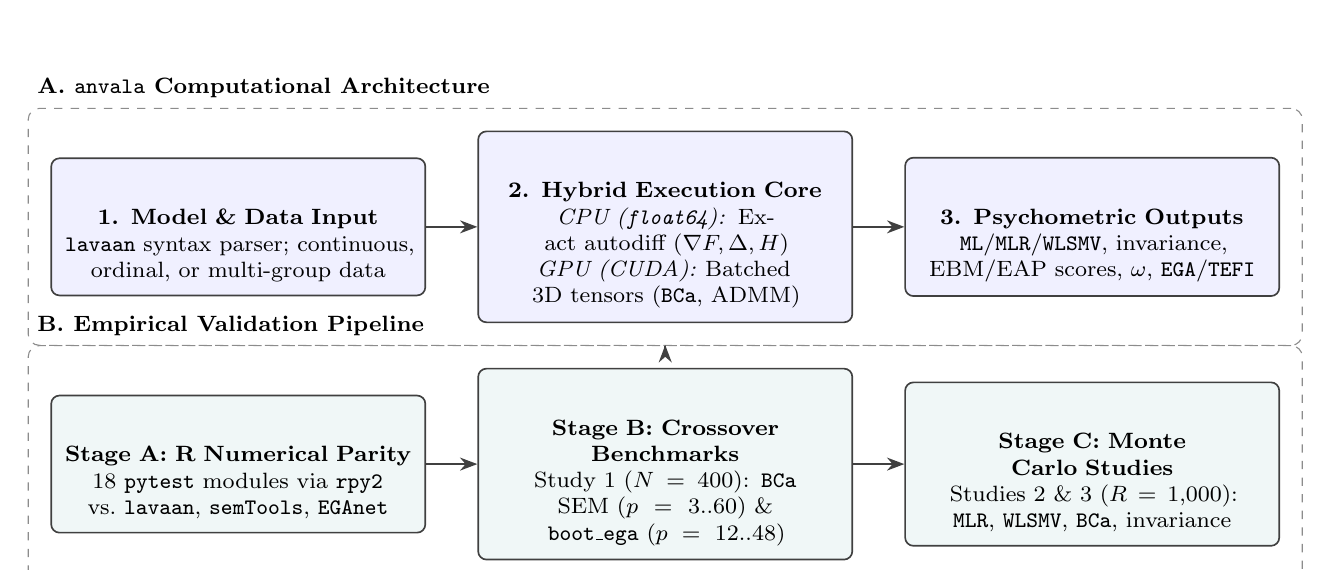
\begin{tikzpicture}[
      font=\footnotesize\singlespacing,
      node distance=0.65cm and 0.65cm,
      box/.style={
        rectangle, rounded corners=3pt, draw=black!75, line width=0.6pt,
        align=center, minimum height=1.35cm, text width=4.4cm, inner sep=5pt
      },
      archbox/.style={box, fill=blue!6},
      valbox/.style={box, fill=teal!6},
      groupbox/.style={
        rectangle, rounded corners=4pt, draw=black!45, dashed, inner sep=8pt
      },
      arrow/.style={-{Stealth[length=2.2mm]}, line width=0.7pt, draw=black!75}
    ]
    
    % --- Camada Superior: Arquitetura do Software ---
    \node[archbox] (input) {
      \textbf{1. Model \& Data Input}\\
      \texttt{lavaan} syntax parser; continuous, ordinal, or multi-group data
    };
    
    \node[archbox, right=of input] (engine) {
      \textbf{2. Hybrid Execution Core}\\
      \textit{CPU (\texttt{float64}):} Exact autodiff ($\nabla F, \Delta, H$)\\
      \textit{GPU (CUDA):} Batched 3D tensors (\texttt{BCa}, ADMM)
    };
    
    \node[archbox, right=of engine] (output) {
      \textbf{3. Psychometric Outputs}\\
      \texttt{ML}/\texttt{MLR}/\texttt{WLSMV}, invariance, EBM/EAP scores, $\omega$, \texttt{EGA}/\texttt{TEFI}
    };
    
    \draw[arrow] (input) -- (engine);
    \draw[arrow] (engine) -- (output);
    
    % --- Camada Inferior: Pipeline de Validação ---
    \node[valbox, below=1.25cm of input] (parity) {
      \textbf{Stage A: R Numerical Parity}\\
      18 \texttt{pytest} modules via \texttt{rpy2} vs.\ \texttt{lavaan}, \texttt{semTools}, \texttt{EGAnet}
    };
    
    \node[valbox, right=of parity] (speed) {
      \textbf{Stage B: Crossover Benchmarks}\\
      Study 1 ($N=400$): \texttt{BCa} SEM ($p=3..60$) \& \texttt{boot\_ega} ($p=12..48$)
    };
    
    \node[valbox, right=of speed] (mc) {
      \textbf{Stage C: Monte Carlo Studies}\\
      Studies 2 \& 3 ($R=1{,}000$): \texttt{MLR}, \texttt{WLSMV}, \texttt{BCa}, invariance
    };
    
    \draw[arrow] (parity) -- (speed);
    \draw[arrow] (speed) -- (mc);
    
    % --- Caixas de Agrupamento ---
    \begin{scope}[on background layer]
      \node[groupbox, fit=(input)(engine)(output), label={[font=\footnotesize\bfseries, anchor=south west]north west:A. \texttt{anvala} Computational Architecture}] (g1) {};
      \node[groupbox, fit=(parity)(speed)(mc), label={[font=\footnotesize\bfseries, anchor=south west]north west:B. Empirical Validation Pipeline}] (g2) {};
    \end{scope}
    
    \draw[arrow, dashed] (g1.south) -- (g2.north);
    
    \end{tikzpicture}
    \caption{Overview of the \texttt{anvala} Hybrid CPU--GPU Computational Architecture (Panel A) and Three-Stage Numerical and Monte Carlo Validation Pipeline (Panel B)}
    \label{fig:workflow}
\end{figure}

% ==================== RESULTS ====================
\section{Results}

\subsection{Stage A: Numerical Parity Against R Reference Packages}

Table~\ref{tab:parity} summarizes side-by-side numerical comparisons between R reference packages and \texttt{anvala} across canonical continuous, robust, structural, ordinal, multi-group, bifactor, and network psychometric models. Across all normal-theory ML and ordinal WLSMV factor models, parameter estimates, polychoric thresholds, and bifactor indices agreed with \texttt{lavaan} and \texttt{BifactorIndicesCalculator} within $1.11 \times 10^{-16}$ to $1.99 \times 10^{-6}$. Robust sandwich standard errors and Yuan--Bentler/Satorra--Bentler scaled test statistics in \texttt{MLR} and multi-group invariance models agreed within $1.75 \times 10^{-5}$ to $1.81 \times 10^{-5}$, while the full Political Democracy structural equation model ($N = 75$) matched focal path estimates and fit indices to five decimal places ($\max|\Delta| = 1.10 \times 10^{-4}$ across all free parameters and standard errors). In network psychometrics, \texttt{anvala} recovered the exact same three-factor community partition as \texttt{EGAnet}, matched the Total Entropy Fit Index to machine precision ($\Delta = 8.88 \times 10^{-16}$), and reproduced the full $9 \times 9$ \texttt{EBICglasso} partial correlation matrix within $\max|\Delta| = 2.54 \times 10^{-6}$.

\begin{table}[htbp]
    \centering
    \caption{Stage A Numerical Parity Benchmark Comparing R Reference Packages and \texttt{anvala} Across Canonical Models}
    \label{tab:parity}
    \resizebox{\textwidth}{!}{%
    \begin{tabular}{llllllr}
    \toprule
    Domain & Dataset & R Reference & Metric & R Value & \texttt{anvala} Value & $\max|\Delta|$ \\
    \midrule
    CFA (\texttt{ML}) & HS1939 ($N=301$) & \texttt{lavaan} 0.7-2 & $\lambda(\text{visual} \sim \text{x2})$ & 0.55350 & 0.55350 & $8.93 \times 10^{-7}$ \\
     & & & $\chi^2$ ($\text{df}=24$) & 85.30552 & 85.30552 & $8.93 \times 10^{-7}$ \\
     & & & CFI / RMSEA & 0.93056 / 0.09212 & 0.93056 / 0.09212 & $8.93 \times 10^{-7}$ \\
    CFA (\texttt{MLR}) & HS1939 ($N=301$) & \texttt{lavaan} 0.7-2 & Sandwich SE ($\text{x2}$) & 0.13208 & 0.13208 & $1.81 \times 10^{-5}$ \\
     & & & Scaled $\chi^2$ / Robust CFI & 87.13160 / 0.92986 & 87.13159 / 0.92986 & $1.81 \times 10^{-5}$ \\
    SEM (\texttt{ML}) & PolDem ($N=75$) & \texttt{lavaan} 0.7-2 & $\text{dem65} \sim \text{dem60}$ (SE) & 0.83734 (0.09835) & 0.83734 (0.09835) & $1.10 \times 10^{-4}$ \\
     & & & $\chi^2$ / CFI & 38.12522 / 0.99537 & 38.12522 / 0.99537 & $1.10 \times 10^{-4}$ \\
    Ordinal (\texttt{WLSMV}) & HS1939-Ord & \texttt{lavaan} 0.7-2 & $\lambda(\text{visual} \sim \text{x2})$ & 0.52992 & 0.52992 & $6.87 \times 10^{-8}$ \\
     & & & Scaled $\chi^2$ / Robust CFI & 83.38528 / 0.91790 & 83.38528 / 0.91790 & $1.99 \times 10^{-6}$ \\
    Multi-Group (\texttt{MLR}) & HS1939 ($G=2$) & \texttt{lavaan} 0.7-2 & Scalar Scaled $\chi^2$ / CFI & 166.74822 / 0.88115 & 166.74820 / 0.88115 & $1.75 \times 10^{-5}$ \\
    Bifactor Indices & HS1939 ($N=301$) & \texttt{BifactorIndices} & ECV / PUC / $\omega_H$ & 0.34444 / 0.75000 / 0.54680 & 0.34444 / 0.75000 / 0.54680 & $1.11 \times 10^{-16}$ \\
    Network (\texttt{EGA}) & HS1939 ($N=301$) & \texttt{EGAnet} 2.4.1 & Dimensions ($K$) / TEFI & 3 / $-5.15041$ & 3 / $-5.15041$ & $8.88 \times 10^{-16}$ \\
     & & & $9 \times 9$ Partial Corr. Matrix & 36 unique edges & 36 unique edges & $2.54 \times 10^{-6}$ \\
    \bottomrule
    \end{tabular}%
    }
    \vspace{4pt}
    \par\noindent\footnotesize\textit{Note.} $\max|\Delta|$ denotes the maximum absolute discrepancy across the full vector of parameters, standard errors, thresholds, or fit indices in each benchmark module. HS1939 = Holzinger--Swineford (1939) dataset; PolDem = Bollen's (1989) Political Democracy dataset.
    \end{table}

\subsection{Study 1: Computational Scalability and CPU--GPU Crossover Benchmarks}

Table~\ref{tab:study1} reports wall-clock execution times across bootstrap replications ($B$) and indicator dimensionalities ($p$) compared against both single-core and 6-core R baselines. In Study 1A ($p = 3$ path mediation), vectorized CPU execution in \texttt{anvala} completed $B = 5{,}000$ \texttt{BCa} resamples in $0.68\text{ s}$ ($151.50\times$ faster than 1-core \texttt{lavaan} and $33.24\times$ faster than 6-core \texttt{lavaan}), outperforming CUDA execution ($1.27\text{ s}$) because the $360\text{ KB}$ covariance tensor fits inside CPU L2/L3 cache.

Study 1B ($B = 1{,}000$ latent variable mediation across $p \in \{6, 15, 30, 60\}$) identified the exact empirical crossover point between CPU and GPU execution within Python. At $p = 6$ indicators, CPU ($3.51\text{ s}$) and RTX 3060 GPU ($3.58\text{ s}$) performed identically while outperforming both 1-core ($19.07\text{ s}$) and 6-core ($5.07\text{ s}$) \texttt{lavaan}. At $p = 15$ indicators (a standard three-factor, five-item-per-factor structural model), GPU tensor batching ($9.49\text{ s}$) overtook Python CPU execution ($11.18\text{ s}$) and remained $2.26\times$ faster than default 1-core \texttt{lavaan} ($21.47\text{ s}$). At higher dimensionalities ($p = 30$ and $p = 60$), GPU batching accelerated Python execution by $2.03\times$ ($29.44\text{ s}$ vs.\ $59.84\text{ s}$) and $7.28\times$ ($103.98\text{ s}$ vs.\ $756.59\text{ s}$), whereas \texttt{lavaan}'s compiled C++ analytical Jacobians scaled more gradually ($26.64\text{ s}$ and $52.53\text{ s}$ on 1 core).

A parallel trade-off emerged in \texttt{boot\_ega} (Studies 1C and 1D). At $p = 12$ indicators (Study 1C), GPU batching accelerated \texttt{anvala} by $12.94\times$ to $21.65\times$ over 1-core Python CPU ($3.98\text{ s}$ to $23.90\text{ s}$ vs.\ $51.53\text{ s}$ to $517.52\text{ s}$; $19.46\text{ s}$ on the NVIDIA L4 at $B = 1{,}000$) and matched or exceeded 1-core \texttt{EGAnet} up to $B = 250$ ($3.98\text{ s}$ vs.\ $10.34\text{ s}$ at $B = 100$). When network dimensionality increased to $p = 24$ and $p = 48$ (Study 1D), dense \texttt{float64} $O(p^3)$ eigendecompositions across $L = 100$ penalties increased RTX 3060 execution time to $59.68\text{ s}$ and $2{,}267.65\text{ s}$, whereas \texttt{EGAnet}'s compiled Fortran coordinate-descent solver (\texttt{glasso}) completed $B = 500$ in $17.85\text{ s}$ and $115.86\text{ s}$ on 1 core ($9.04\text{ s}$ and $26.93\text{ s}$ on 6 cores).

\begin{table}[htbp]
\centering
\caption{Study 1 Wall-Clock Execution Times (in Seconds) Across Resampling Grid ($B$), Model Dimensionality ($p$), and CPU/GPU Hardware ($N = 400$)}
\label{tab:study1}
\footnotesize
\setlength{\tabcolsep}{3.6pt}
\begin{tabular}{lrrrrrrrr}
\toprule
Benchmark / Condition & $p$ & $B$ & R (1 Core) & R (6 Cores) & \texttt{anvala} CPU & \texttt{anvala} GPU & GPU vs. CPU & GPU vs. R (1c) \\
\midrule
\multicolumn{9}{l}{\textit{Study 1A: SEM Path Mediation (\texttt{BCa}, Varying $B$)}} \\
Observed mediation & 3 & 250 & 5.23 & 3.09 & 0.16 & 0.24 & $0.68\times$ & $21.88\times$ \\
 & 3 & 500 & 10.74 & 3.26 & 0.13 & 0.34 & $0.38\times$ & $31.91\times$ \\
 & 3 & 1,000 & 21.17 & 5.37 & 0.18 & 0.46 & $0.39\times$ & $45.87\times$ \\
 & 3 & 2,000 & 41.41 & 9.86 & 0.30 & 0.64 & $0.47\times$ & $64.66\times$ \\
 & 3 & 5,000 & 103.18 & 22.64 & 0.68 & 1.27 & $0.54\times$ & $81.33\times$ \\
\addlinespace
\multicolumn{9}{l}{\textit{Study 1B: Three-Factor Latent Mediation (\texttt{BCa}, Empirical CPU--GPU Crossover)}} \\
2 items/factor & 6 & 1,000 & 19.07 & 5.07 & 3.51 & 3.58 & $0.98\times$ & $5.32\times$ \\
5 items/factor (crossover) & 15 & 1,000 & 21.47 & 5.63 & 11.18 & 9.49 & $1.18\times$ & $2.26\times$ \\
10 items/factor & 30 & 1,000 & 26.64 & 6.62 & 59.84 & 29.44 & $2.03\times$ & $0.90\times$ \\
20 items/factor & 60 & 1,000 & 52.53 & 12.72 & 756.59 & 103.98 & $7.28\times$ & $0.51\times$ \\
\addlinespace
\multicolumn{9}{l}{\textit{Study 1C: Nonparametric \texttt{boot\_ega} (Three Communities, Varying $B$)}} \\
12-item network & 12 & 100 & 10.34 & 9.64 & 51.53 & 3.98 & $12.94\times$ & $2.60\times$ \\
 & 12 & 250 & 6.58 & 7.00 & 128.84 & 6.02 & $21.39\times$ & $1.09\times$ \\
 & 12 & 500 & 9.60 & 9.41 & 261.70 & 12.07 & $21.68\times$ & $0.80\times$ \\
 & 12 & 1,000 & 17.42 & 9.30 & 517.52 & 23.90 & $21.65\times$ & $0.73\times$ \\
\addlinespace
\multicolumn{9}{l}{\textit{Study 1D: Nonparametric \texttt{boot\_ega} Dimensionality Scaling ($O(p^3)$)}} \\
3 communities $\times$ 4 items & 12 & 500 & 13.78 & 10.21 & --- & 11.18 & --- & $1.23\times$ \\
3 communities $\times$ 8 items & 24 & 500 & 17.85 & 9.04 & --- & 59.68 & --- & $0.30\times$ \\
3 communities $\times$ 16 items & 48 & 500 & 115.86 & 26.93 & --- & 2,267.65 & --- & $0.05\times$ \\
\bottomrule
\end{tabular}
\vspace{4pt}
\par\noindent\footnotesize\textit{Note.} Workstation timings recorded on Intel Core i5-10400F (6 physical cores, PyTorch \texttt{num\_threads = 6}) and NVIDIA GeForce RTX 3060 (12 GB VRAM). Multi-core R timings used \texttt{parallel = "snow", ncpus = 6} in \texttt{lavaan} and \texttt{ncores = 6} in \texttt{EGAnet::bootEGA}. Studies 1C and 1D on the workstation used nonparametric resampling (\texttt{boot\_type = "nonparametric"}), whereas the cloud NVIDIA L4 benchmark ($B = 5{,}000$ path mediation in $0.79\text{ s}$; $B = 1{,}000$ \texttt{boot\_ega} at $p = 12$ in $19.46\text{ s}$, $32.77\times$ faster than CPU) used parametric resampling. Each R baseline ran inside a fresh \texttt{Rscript} subprocess; fixed package loading, PSOCK cluster initialization, and bytecode JIT compilation overhead ($\approx 6\text{--}9\text{ s}$) accounts for the flat scaling of \texttt{EGAnet::bootEGA} across small $B \in \{100, 250\}$.
\end{table}

\subsection{Study 2: Monte Carlo Parameter Recovery and Interval Coverage}

Across all 36 cells of Study 2 ($R = 1{,}000$ replications per cell), \texttt{anvala} achieved a $100\%$ convergence rate without non-positive-definite covariance warnings. As summarized in Table~\ref{tab:study2}, relative parameter bias remained negligible across all estimators and sample sizes, well below the $5\%$ benchmark recommended for covariance structure simulations \parencite{hoogland1998}. Under severe non-normality with \texttt{MLR} (Study 2A), relative bias ranged from $-0.68\%$ to $+1.39\%$ at $N = 150$, $-1.07\%$ to $+0.77\%$ at $N = 300$, and $-0.44\%$ to $+0.47\%$ at $N = 600$. Sandwich standard errors tracked empirical sampling variability closely ($\overline{\mathrm{SE}}/\mathrm{SD}$ between $0.94$ and $1.04$), yielding empirical 95\% confidence interval coverage between $92.1\%$ and $95.1\%$.

Under ordinal \texttt{WLSMV} estimation (Study 2B), polychoric factor loadings exhibited relative bias within $-0.17\%$ to $+1.23\%$ at $N = 150$ and within $\pm 0.22\%$ at $N \ge 300$, with $\overline{\mathrm{SE}}/\mathrm{SD}$ ratios between $0.89$ and $1.04$ and coverage reaching $94.3\%$--$95.2\%$ at $N = 600$. Similarly, in the mediation model (Study 2C), \texttt{BCa} bootstrap intervals accurately recovered the asymmetric indirect effect $ab = 0.225$, with relative bias decreasing from $+1.44\%$ at $N = 150$ to $-0.12\%$ at $N = 300$ and $-0.11\%$ at $N = 600$, while maintaining empirical coverage between $93.8\%$ and $95.1\%$.

\begin{table}[htbp]
\centering
\caption{Study 2 Monte Carlo Parameter Recovery, Standard Error Calibration, and 95\% Confidence Interval Coverage ($R = 1{,}000$ Replications per Cell, $\mathrm{MCSE} = 0.69\%$)}
\label{tab:study2}
\footnotesize
\setlength{\tabcolsep}{4pt}
\begin{tabular}{llrrrrrrrr}
\toprule
Condition / Estimator & Parameter & True & $N$ & Mean Est. & Rel. Bias (\%) & Emp. SD & Mean SE & $\overline{\mathrm{SE}}/\mathrm{SD}$ & Cov. (\%) \\
\midrule
2A: Non-Normal \texttt{MLR} & $\lambda_{12}$ (\texttt{F1 =\textasciitilde{} x2}) & 0.900 & 150 & 0.900 & $0.01$ & 0.143 & 0.140 & 0.98 & 94.8 \\
 & & & 300 & 0.907 & $0.77$ & 0.099 & 0.097 & 0.99 & 94.9 \\
 & & & 600 & 0.904 & $0.47$ & 0.069 & 0.067 & 0.97 & 93.9 \\
 & $\lambda_{13}$ (\texttt{F1 =\textasciitilde{} x3}) & 0.800 & 150 & 0.800 & $0.00$ & 0.136 & 0.128 & 0.94 & 92.9 \\
 & & & 300 & 0.805 & $0.64$ & 0.092 & 0.090 & 0.98 & 94.7 \\
 & & & 600 & 0.802 & $0.20$ & 0.065 & 0.062 & 0.96 & 93.8 \\
 & $\psi_{12}$ (\texttt{F1 \textasciitilde\textasciitilde{} F2}) & 0.256 & 150 & 0.256 & $-0.18$ & 0.082 & 0.083 & 1.01 & 92.9 \\
 & & & 300 & 0.254 & $-0.85$ & 0.060 & 0.059 & 0.99 & 92.4 \\
 & & & 600 & 0.257 & $0.22$ & 0.040 & 0.042 & 1.04 & 95.1 \\
 & $\psi_{11}$ (\texttt{F1 \textasciitilde\textasciitilde{} F1}) & 0.640 & 150 & 0.649 & $1.39$ & 0.167 & 0.164 & 0.98 & 92.1 \\
 & & & 300 & 0.636 & $-0.57$ & 0.121 & 0.116 & 0.96 & 92.1 \\
 & & & 600 & 0.641 & $0.14$ & 0.082 & 0.084 & 1.01 & 94.9 \\
 & $\theta_{22}$ (\texttt{x2 \textasciitilde\textasciitilde{} x2}) & 0.482 & 150 & 0.478 & $-0.68$ & 0.115 & 0.111 & 0.96 & 92.9 \\
 & & & 300 & 0.476 & $-1.07$ & 0.082 & 0.080 & 0.97 & 92.1 \\
 & & & 600 & 0.480 & $-0.44$ & 0.058 & 0.057 & 0.98 & 94.0 \\
\addlinespace
2B: Ordinal \texttt{WLSMV} & $\lambda_1$ (\texttt{F1 =\textasciitilde{} u1}) & 0.650 & 150 & 0.658 & $1.23$ & 0.066 & 0.059 & 0.89 & 90.1 \\
 & & & 300 & 0.651 & $0.22$ & 0.043 & 0.043 & 0.99 & 94.4 \\
 & & & 600 & 0.650 & $0.00$ & 0.030 & 0.031 & 1.01 & 95.2 \\
 & $\lambda_3$ (\texttt{F1 =\textasciitilde{} u3}) & 0.750 & 150 & 0.751 & $0.10$ & 0.053 & 0.050 & 0.94 & 92.9 \\
 & & & 300 & 0.751 & $0.10$ & 0.037 & 0.035 & 0.96 & 93.8 \\
 & & & 600 & 0.751 & $0.11$ & 0.026 & 0.025 & 0.98 & 94.3 \\
 & $\lambda_5$ (\texttt{F1 =\textasciitilde{} u5}) & 0.850 & 150 & 0.849 & $-0.17$ & 0.040 & 0.040 & 1.00 & 94.6 \\
 & & & 300 & 0.852 & $0.19$ & 0.029 & 0.028 & 0.98 & 93.9 \\
 & & & 600 & 0.850 & $-0.03$ & 0.019 & 0.020 & 1.04 & 95.1 \\
\addlinespace
2C: Mediation \texttt{BCa} & $a$ (\texttt{X $\to$ M}) & 0.500 & 150 & 0.504 & $0.74$ & 0.085 & 0.082 & 0.97 & 94.3 \\
 & & & 300 & 0.500 & $-0.04$ & 0.061 & 0.058 & 0.95 & 92.1 \\
 & & & 600 & 0.500 & $-0.09$ & 0.040 & 0.041 & 1.02 & 94.6 \\
 & $b$ (\texttt{M $\to$ Y}) & 0.450 & 150 & 0.453 & $0.55$ & 0.084 & 0.082 & 0.97 & 93.4 \\
 & & & 300 & 0.450 & $-0.01$ & 0.061 & 0.058 & 0.95 & 92.7 \\
 & & & 600 & 0.450 & $-0.05$ & 0.041 & 0.041 & 1.00 & 94.0 \\
 & $c'$ (\texttt{X $\to$ Y}) & 0.200 & 150 & 0.200 & $0.14$ & 0.094 & 0.092 & 0.98 & 93.3 \\
 & & & 300 & 0.201 & $0.57$ & 0.066 & 0.065 & 0.98 & 93.9 \\
 & & & 600 & 0.201 & $0.26$ & 0.046 & 0.046 & 0.99 & 94.0 \\
 & $ab$ (Indirect) & 0.225 & 150 & 0.228 & $1.44$ & 0.059 & 0.057 & 0.96 & 93.8 \\
 & & & 300 & 0.225 & $-0.12$ & 0.040 & 0.039 & 0.97 & 94.0 \\
 & & & 600 & 0.225 & $-0.11$ & 0.028 & 0.028 & 1.00 & 95.1 \\
\bottomrule
\end{tabular}
\vspace{4pt}
\par\noindent\footnotesize\textit{Note.} Convergence rate was $100\%$ across all conditions. Rel. Bias = $100 \times (\bar{\hat{\theta}} - \theta)/\theta$; Emp. SD = empirical standard deviation across replications; Mean SE = mean estimated standard error; Cov. = empirical coverage of nominal 95\% confidence intervals ($\mathrm{MCSE} = \sqrt{0.95 \times 0.05 / 1000} = 0.69\%$).
\end{table}

\subsection{Study 3: Multi-Group Measurement Invariance and Latent Mean Recovery}

Table~\ref{tab:study3ab} summarizes hierarchical invariance test performance across Study 3A (full invariance) and Study 3B (non-invariance on item \texttt{x3}). Under full invariance (Study 3A), Satorra--Bentler scaled $\Delta\chi^2$ tests maintained well-controlled empirical Type I error rates across metric, scalar, and strict constraints at both $N_g = 150$ ($.061$, $.042$, and $.051$, respectively) and $N_g = 300$ ($.059$, $.042$, and $.061$), falling well within Bradley's (\citeyear{bradley1978}) liberal acceptability bounds ($[.025, .075]$). Practical fit criteria based on $\Delta\mathrm{CFI} < -.010$ \parencite{chen2007} exhibited low false-positive rates at $N_g = 150$ ($.043$--$.052$) and near-zero false-positive rates at $N_g = 300$ ($.003$--$.008$), whereas $\Delta\mathrm{RMSEA} > .015$ over-rejected invariant models across both sample sizes ($.080$--$.175$), consistent with known small-sample sampling variability of RMSEA in low-degrees-of-freedom models.

When item \texttt{x3} violated metric and scalar invariance in Group 2 (Study 3B; $\Delta\lambda_3 = -0.30$, $\Delta\nu_3 = +0.50$), statistical power to detect loading non-invariance via $\Delta\chi^2$ reached $.734$ at $N_g = 150$ and $.944$ at $N_g = 300$, while scalar non-invariance was detected with $.999$ and $1.000$ power, respectively. Because the strict invariance model in Study 3B was nested within the misspecified full scalar model, constraining invariant residual variances yielded minor spillover rejection rates ($.096$ and $.141$), confirming specificity to the violated loading and intercept parameters.

\begin{table}[htbp]
\centering
\caption{Study 3A and 3B Multi-Group Measurement Invariance Rejection Rates Under Full Invariance (Type I Error) and Item \texttt{x3} Non-Invariance (Power)}
\label{tab:study3ab}
\footnotesize
\setlength{\tabcolsep}{4.5pt}
\begin{tabular}{llrrrrrrr}
\toprule
Condition & $N_g$ & Transition & $\overline{\Delta\chi^2}$ & $\Delta\chi^2$ ($p < .05$) & $\overline{\Delta\mathrm{CFI}}$ & $\Delta\mathrm{CFI} < -.010$ & $\overline{\Delta\mathrm{RMSEA}}$ & $\Delta\mathrm{RMSEA} > .015$ \\
\midrule
3A: Full Invariance & 150 & Metric & 3.19 & .061 & $-.001$ & .044 & $-.002$ & .175 \\
 & & Scalar & 3.06 & .042 & $-.001$ & .043 & $-.002$ & .113 \\
 & & Strict & 4.09 & .051 & $-.001$ & .052 & $-.001$ & .132 \\
 & 300 & Metric & 3.11 & .059 & $-.001$ & .004 & $-.001$ & .149 \\
 & & Scalar & 2.87 & .042 & $-.000$ & .003 & $-.002$ & .080 \\
 & & Strict & 4.02 & .061 & $-.000$ & .008 & $-.001$ & .096 \\
\addlinespace
3B: Non-Invariance & 150 & Metric & 12.25 & .734 & $-.020$ & .728 & .061 & .833 \\
 & & Scalar & 31.92 & .999 & $-.071$ & .999 & .071 & .980 \\
 & & Strict & 4.65 & .096 & $-.002$ & .135 & $-.023$ & .000 \\
 & 300 & Metric & 20.39 & .944 & $-.020$ & .824 & .072 & .962 \\
 & & Scalar & 63.07 & 1.000 & $-.074$ & 1.000 & .073 & .997 \\
 & & Strict & 5.39 & .141 & $-.002$ & .060 & $-.024$ & .000 \\
\bottomrule
\end{tabular}
\vspace{4pt}
\par\noindent\footnotesize\textit{Note.} $N_g$ = sample size per group ($G = 2$ groups, $R = 1{,}000$ replications per cell, $\mathrm{MCSE} = 0.69\%$ at nominal $\alpha = .05$). In Study 3B, Group 2 parameters for item \texttt{x3} were shifted by $\Delta\lambda_3 = -0.30$ and $\Delta\nu_3 = +0.50$.
\end{table}

Finally, Study 3C demonstrated the practical consequence of ignoring partial invariance when estimating latent group mean differences ($\kappa_2 = 0.400$; Table~\ref{tab:study3c}). Imposing a misspecified full scalar invariance model inflated the estimated latent mean difference to $0.459$ ($+14.65\%$ relative bias) at $N_g = 150$ and $0.479$ ($+19.69\%$ relative bias) at $N_g = 300$, degrading 95\% confidence interval coverage to $89.0\%$ and $78.5\%$, respectively. Freeing the non-invariant loading and intercept of item \texttt{x3} via \texttt{group\_partial} eliminated this distortion, recovering $\hat{\kappa}_2 = 0.387$ ($-3.16\%$ bias, $94.0\%$ coverage) at $N_g = 150$ and $\hat{\kappa}_2 = 0.410$ ($+2.53\%$ bias, $94.5\%$ coverage) at $N_g = 300$.

\begin{table}[htbp]
    \centering
    \caption{Study 3C Recovery of Group 2 Latent Mean ($\kappa_2 = 0.400$) Under Misspecified Full Scalar vs. Partial Scalar Invariance}
    \label{tab:study3c}
    \footnotesize
    \begin{tabular}{llrrrrr}
    \toprule
    Model Specification & $N_g$ & Mean Est. & Rel. Bias (\%) & Mean SE & RMSE & 95\% Cov. (\%) \\
    \midrule
    Full Scalar (Misspecified) & 150 & 0.4586 & $+14.65$ & 0.1005 & 0.1188 & 89.0 \\
    Partial Scalar (\texttt{group\_partial}) & 150 & 0.3874 & $-3.16$ & 0.1027 & 0.1049 & 94.0 \\
    \addlinespace
    Full Scalar (Misspecified) & 300 & 0.4787 & $+19.69$ & 0.0716 & 0.1102 & 78.5 \\
    Partial Scalar (\texttt{group\_partial}) & 300 & 0.4101 & $+2.53$ & 0.0731 & 0.0793 & 94.5 \\
    \bottomrule
    \end{tabular}
    \vspace{4pt}
    \par\noindent\footnotesize\textit{Note.} True population latent mean difference $\kappa_2 = 0.400$ on the \texttt{x1} marker metric ($R = 1{,}000$ replications per cell, $\mathrm{MCSE} = 0.69\%$). Partial scalar models freed \texttt{F1 =\textasciitilde{} x3} and \texttt{x3 \textasciitilde{} 1} across groups.
    \end{table}


% ==================== DISCUSSION ====================
\section{Discussion}

The present work introduced \texttt{anvala} (v0.1.0), an open-source Python library designed to provide R-equivalent latent variable and network psychometrics natively inside the PyTorch ecosystem. Across canonical integration benchmarks and three simulation studies, \texttt{anvala} matched R reference packages---\texttt{lavaan} (v0.7-2), \texttt{semTools} (v0.5-9), \texttt{EGAnet} (v2.4.1), and \texttt{BifactorIndicesCalculator} (v0.2.2)---within $10^{-16}$ to $10^{-5}$ while achieving $100\%$ convergence, negligible parameter bias ($< 5\%$), well-calibrated standard errors, and substantial GPU speedups for resampling workflows within Python.

Study 1 revealed clear architectural trade-offs across model dimensionalities ($p$) and hardware backends that translate directly into practical usage guidelines. In low-dimensional path mediation ($p = 3$, $q = 6$), stacking $B = 5{,}000$ double-precision (\texttt{float64}) covariance matrices yields a $360\text{ KB}$ tensor that resides inside CPU L2/L3 cache; consequently, vectorized CPU execution completed $5{,}000$ \texttt{BCa} resamples in $0.68\text{ s}$ ($151.50\times$ faster than 1-core \texttt{lavaan}), outperforming CUDA execution ($1.27\text{ s}$) by avoiding host-to-device memory transfer overhead. Expanding to latent variable mediation (Study 1B) pinpointed the empirical crossover at $p = 15$ indicators (a standard three-factor, five-item-per-factor model), where GPU batching ($9.49\text{ s}$) overtook Python CPU execution ($11.18\text{ s}$) and remained $2.26\times$ faster than default 1-core \texttt{lavaan} ($21.47\text{ s}$). At larger dimensionalities ($p = 30, 60$), GPU batching continued to accelerate Python execution by $2.03\times$ to $7.28\times$ over CPU, whereas \texttt{lavaan}'s compiled C++ analytical Kronecker Jacobians scaled more gradually than \texttt{anvala}'s general-purpose automatic-differentiation Jacobian tensor $\mathbf{J} \in \mathbb{R}^{B \times m \times q}$. A parallel distinction emerged in \texttt{boot\_ega} (Studies 1C and 1D): on typical psychometric scales ($p = 12$), GPU tensor batching accelerated Python execution by $21.65\times$ on the RTX 3060 and $32.77\times$ on the NVIDIA L4, whereas on large item pools ($p = 24, 48$), dense \texttt{float64} $O(p^3)$ eigendecompositions across $L = 100$ penalties (combined with hardware \texttt{float64} rate limits on consumer GeForce GPUs) made compiled Fortran coordinate descent in \texttt{EGAnet::bootEGA} faster in absolute wall-clock time. Researchers should therefore retain the default CPU path for single-model fits and small low-dimensional bootstrap models ($p < 15$), select \texttt{device="cuda"} for bootstrap latent variable models ($p \ge 15$) and standard-scale network stability ($p \le 15$) inside Python pipelines, and rely on compiled R backends when running massive bootstrap grids on high-dimensional networks ($p \ge 24$) outside Python workflows.

Studies 2 and 3 confirmed that these computational gains preserve finite-sample statistical rigor under challenging data conditions. Under severe non-normality (\texttt{MLR}), coarse four-category ordinal discretization (\texttt{WLSMV}), and asymmetric mediation effects (\texttt{BCa}), empirical coverage remained close to the nominal $95\%$ level even at $N = 150$. Moreover, Study 3 underscored two substantive methodological lessons for applied multi-group research. First, under full invariance (Study 3A), the $\Delta\mathrm{RMSEA} > .015$ cutoff \parencite{chen2007} over-rejected invariant models at $N_g = 150$, reflecting the well-documented sampling instability of RMSEA in models with small degrees of freedom \parencite{kenny2015}, whereas Satorra--Bentler $\Delta\chi^2$ tests and $\Delta\mathrm{CFI} < -.010$ maintained well-controlled Type I error rates. Second, Study 3C showed that leaving even a single non-invariant item constrained in a four-indicator scale inflated the estimated latent group mean difference by $19.69\%$ and degraded interval coverage to $78.5\%$ at $N_g = 300$, whereas freeing the offending item via \texttt{group\_partial} reduced bias to $2.53\%$ and restored $94.5\%$ coverage.

From a broader methodological perspective, embedding R-equivalent latent variable and network psychometrics natively inside PyTorch closes a critical bottleneck in generative and computational psychometrics \parencite{russelllasalandra2026, vondavier2021}. Pipelines that generate candidate items with language models, extract dense semantic embeddings, screen local dependence via Unique Variable Analysis (\texttt{uva}), evaluate network dimensionality (\texttt{ega} and \texttt{tefi}), and validate ordinal factor structures (\texttt{WLSMV}) can now execute within a single Python runtime without disk serialization or foreign-function bridges. Furthermore, maintaining an automated \texttt{pytest}--\texttt{rpy2} parity suite against CRAN reference packages establishes a reproducible continuous-integration safeguard against silent numerical drift as underlying tensor libraries evolve.

Several limitations of the current release (v0.1.0) outline clear priorities for future development. First, missing-data handling currently relies on complete cases or user-supplied sufficient matrices rather than Full Information Maximum Likelihood (FIML) estimation, which will be added in an upcoming release to support incomplete continuous datasets under missing-at-random mechanisms. Second, \texttt{anvala} does not yet support multilevel (two-level) SEM or nonlinear latent variable interaction terms. Third, future releases will implement matrix-free Gauss--Newton--Krylov solvers (\texttt{jvp}/\texttt{vjp}) and continuation warm-starts across the $\lambda_l$ regularization grid to reduce memory bandwidth and eigendecomposition overhead in high-dimensional ($p > 24$) GPU resampling. Finally, GPU resampling currently dispatches the full $B \times L$ tensor batch in a single pass; implementing automatic memory-aware chunking will prevent out-of-memory errors when users combine large item pools with dense bootstrap grids on entry-level GPUs.

% ==================== OPEN PRACTICES (MANDATORY BRM) ====================
\section*{Open Practices}
The \texttt{anvala} package (v0.1.0), integration test suite, benchmark scripts, Monte Carlo simulation scripts, and all generated raw datasets are openly available at \url{https://github.com/FredPedrosa/anvala} (archived at Zenodo, DOI: \url{https://doi.org/10.5281/zenodo.24507587}) and via the Python Package Index (\url{https://pypi.org/project/anvala/}). None of the computational studies reported here were preregistered.

% ==================== ACKNOWLEDGMENTS (MANDATORY BRM) ====================
\section*{Acknowledgments}
The author thanks the Conselho Nacional de Desenvolvimento Científico e Tecnológico (CNPq, Brazil) for research fellowship support.

% ==================== DECLARATIONS (MANDATORY BRM) ====================
\section*{Declarations}

\noindent \textbf{Funding.} This research was supported by the Conselho Nacional de Desenvolvimento Científico e Tecnológico (CNPq, Brazil).

\noindent \textbf{Conflicts of interest/Competing interests.} The author has no competing interests to declare that are relevant to the content of this article.

\noindent \textbf{Ethics approval.} Not applicable.

\noindent \textbf{Consent to participate.} Not applicable.

\noindent \textbf{Consent for publication.} Not applicable.

\noindent \textbf{Availability of data and materials.} All synthetic benchmark datasets and Monte Carlo simulation outputs generated and analyzed during the current study are publicly available in the GitHub repository (\url{https://github.com/FredPedrosa/anvala/tree/main/simulations/results}) and archived via Zenodo (\url{https://doi.org/10.5281/zenodo.24507587}).

\noindent \textbf{Code availability.} The source code for \texttt{anvala} (v0.1.0) and all reproducible benchmark and Monte Carlo scripts are available under the MIT License at \url{https://github.com/FredPedrosa/anvala} and installable via PyPI (\texttt{pip install anvala}).

\noindent \textbf{Authors' contributions.} Frederico Gonçalves Pedrosa conceived the software architecture, implemented the package, designed and executed the numerical parity and Monte Carlo simulation studies, and wrote the manuscript.

\noindent \textbf{Declaration of generative AI and AI-assisted technologies.} During the preparation of this work, the author used generative AI tools (Google Gemini and Cursor) to assist with English language editing, \LaTeX{} typesetting, and software refactoring. After using these tools, the author reviewed, verified, and edited all code and manuscript text, and takes full responsibility for the content of the published article.

% ==================== REFERENCES ====================
\printbibliography

\end{document}
